\section{Experiments}\label{sec:experiment}
In this section, we study our solutions for $k$-Sketch query processing
in both offline and online scenarios using the following 
four real datasets. The statistics of these datasets are 
summarized in Table~\ref{tbl:dataset}.

\noindent\textbf{NBA}\footnote{http://www.nba.com} contains the game records for each NBA player from year $1985$ to $2013$. Among all the records, we pick $1,000$ players with at least $200$ game records. In total, we obtain a dataset with $569$K events.

\noindent\textbf{POWER}~\cite{Lichman2013} contains the electricity usage for 370 households between Dec. 2006 and Nov. 2010. Each household is treated as a subject with the daily power usage as an event. In total, there are 1.4M events.

\noindent\textbf{PEMS}~\cite{choe2002freeway} contains the occupancy rate of freeway in San Francisco bay area from Jan. 2008 to Mar. 2009. Each freeway is a subject with the daily occupancy rate as an event. The dataset contains 963 freeways with 5.7M events.

\noindent\textbf{STOCK} contains the hourly price tick for 318 stocks from Mar. 2013 to Feb. 2015.
The dataset is crawled from Yahoo! Finance\footnote{https://finance.yahoo.com/} and contains 2.3M events.

 
\begin{table}[h]
\caption{Statistics of datasets used in the experiments.}
\centering
\begin{tabular}{|c|c|c|c|}
\hline
DataSet & Total Events & Total Subjects  & Longest Sequence \\
\hline
NBA & 569,253 & 1,015&  1,476 \\
\hline
POWER & 1,480,000 & 370 & 4,000 \\
\hline
PEMS & 5,798,918 & 963&  6,149 \\
\hline
STOCK & 2,326,632 & 318&  10,420 \\
\hline
\end{tabular}
\label{tbl:dataset}
\end{table}

In our efficiency study, we evaluate three parameters: (1) $p\in[20,200]$, which refers to the threshold of the ranked-streaks, (2) $k\in[20,100]$, which refers to the size of a sketch and (3) $h\in[20,100]$, which refers to the percentage of historical events for scalability test, i.e. $|\mathbb{H}|h\%$ events are used in the experiments. We do not evaluate the performance with respect to $\alpha$ since $\alpha$ does not impact the running time. We use $p=200$, $h=100$, and $k=20$ as the default values.

All the experiments are conducted on a desktop machine equipped with an Intel i7 Dual-Core 3.0GHz CPU, 8GB memory and 160 GB hard drive. All algorithms are implemented in Java 7. 
 
\subsection{Offline $k$-Sketch Query Processing}
\label{subsec:exp-offline}
Our offline $k$-Sketch query processing algorithms consist of two functional components, \emph{Ranked-streak Generation}
and \emph{Sketch Discovery}. In the ranked-streak generation, we report the performance with varying $p$ and $h$. In the sketch discovery, we report the performance with varying $k$.

\subsubsection{Ranked-Streak Generation Algorithms}
To evaluate the performance, we design the following four methods for comparison:

\noindent\textbf{Brute Force (BF)}. BF exhaustively computes and compares for each subject all the possible streak lengths. 

\noindent\textbf{Visiting Streak Pruning (V-SP)}. V-SP only adopts the \emph{visiting-streak} bound for pruning.

\noindent\textbf{Unseen Streak Pruning (U-SP)}. U-SP only adopts the \emph{unseen-streak} bound for pruning. 

\noindent\textbf{Unseen+Visiting Streak Pruning (UV-SP)}. UV-SP adopts both \emph{unseen-streak} and \emph{visiting-streak} bounds for pruning.

%\subsubsection{Candidate themes generation with varying $p$}
%The running time of the four algorithms in ranked streak generation wrt. $p$ is shown in Fig.~\ref{exp:offline_performance_vary_p}. It is evident that when $p$ increases, more candidate themes are qualified and thus all four algorithms require more computation time. The effect of the two proposed window-based pruning techniques can also be observed from the figure. The insight is that the unseen-window pruning plays a more important role in reducing the running time. Furthermore, when both pruning techniques are used, our method achieves at least two orders of magnitude of performance improvement.
\subsubsection{Ranked-Streaks Generation varying $p$}
The running time of the four algorithms in ranked-streak generation with respect to $p$ is shown in Figure~\ref{exp:offline_performance_vary_p}. It is evident that when $p$ increases, more ranked-streaks are qualified and thus all four algorithms require more computation time. The effect of the two proposed streak-based pruning techniques can also be observed from the figure. The insight is that the unseen-streak pruning plays a more important role in reducing the running time. Furthermore, when both pruning techniques are used, our method (UV-SP) achieves at least two orders of magnitude of performance improvement.

\begin{figure}[t]
\centering
    \begin{subfigure}[b]{0.45\textwidth}
        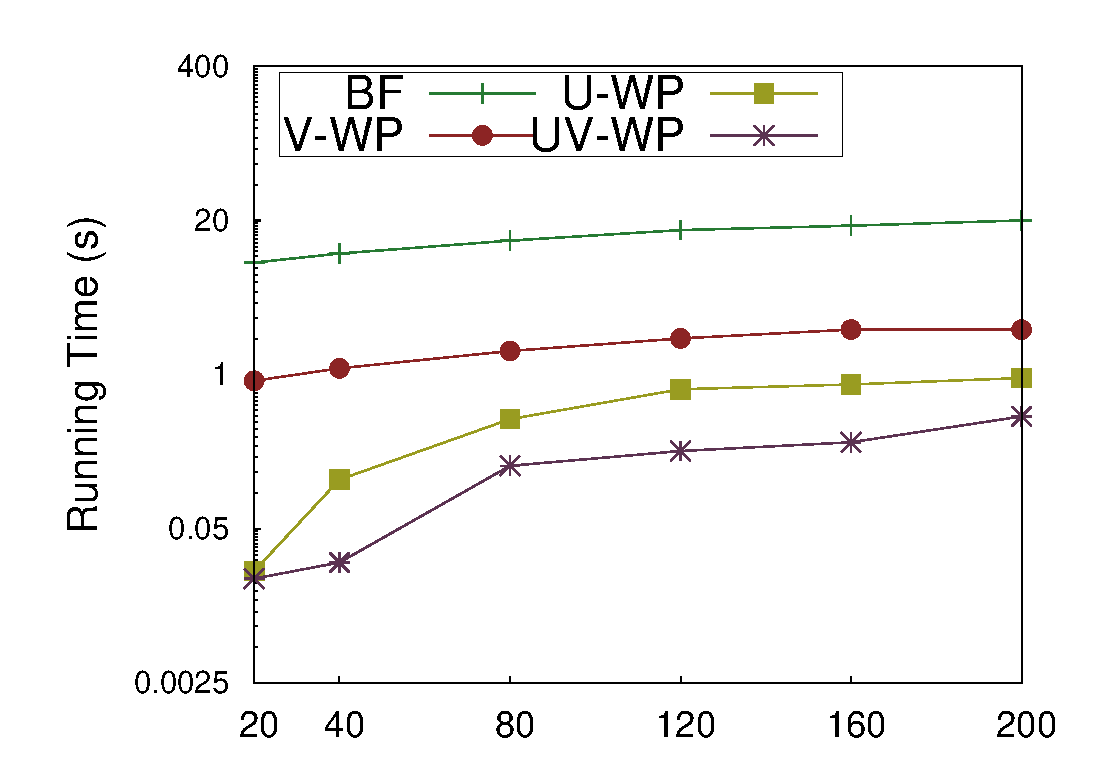
\includegraphics[width=\textwidth]{chapter4/exp/offline/varyp/nba_vary_p.eps}
        \caption{NBA}
    \end{subfigure}
    \begin{subfigure}[b]{0.45\textwidth}
        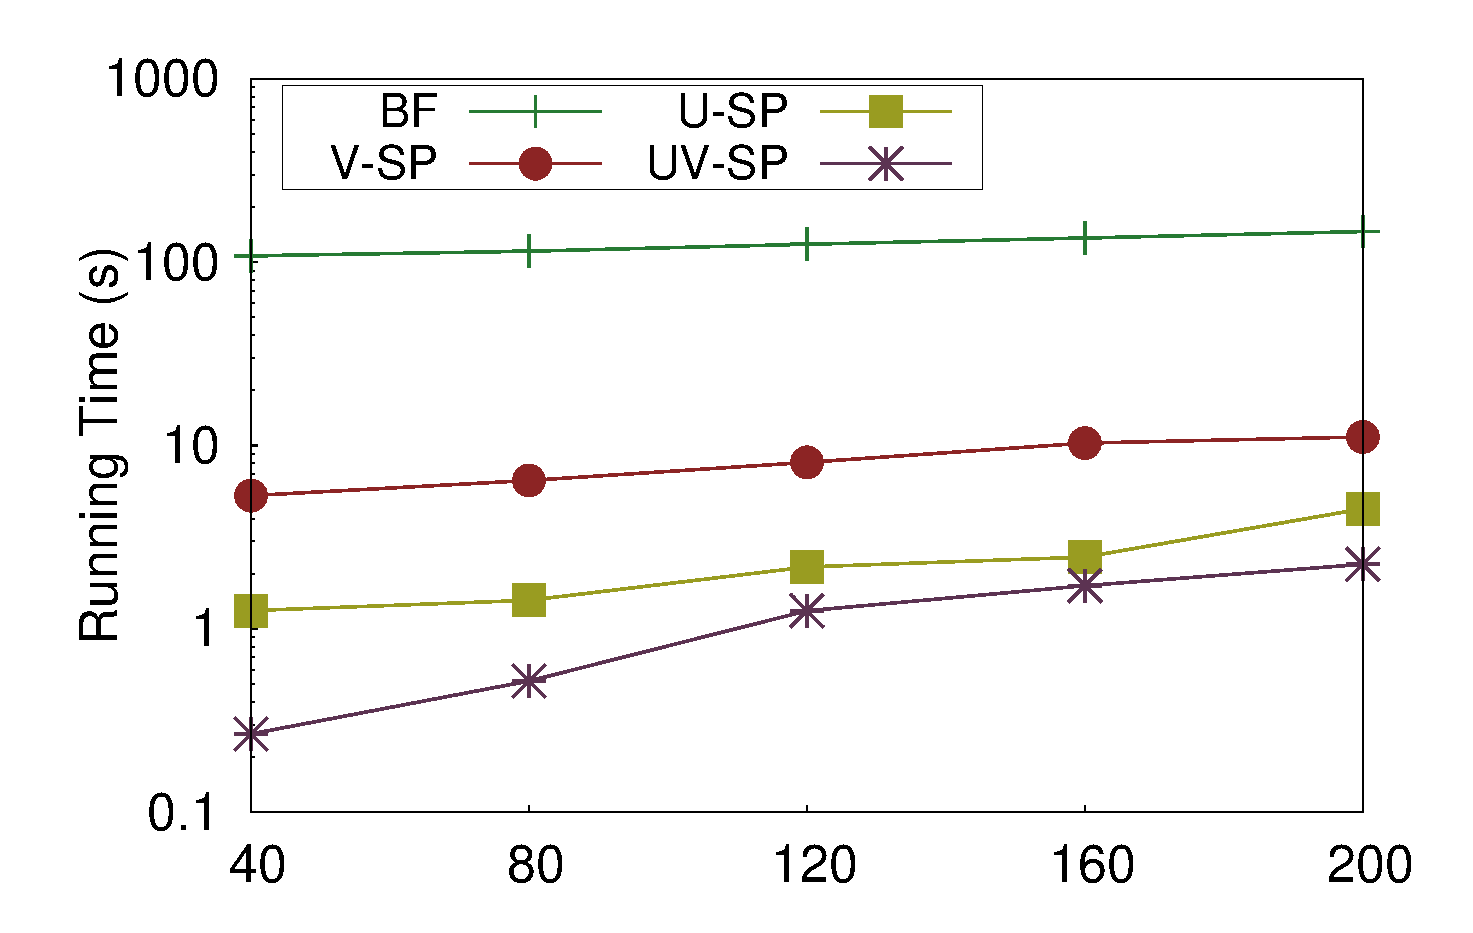
\includegraphics[width=\textwidth]{chapter4/exp/offline/varyp/power_vary_p.eps}
        \caption{POWER}
    \end{subfigure}
    \begin{subfigure}[b]{0.45\textwidth}
        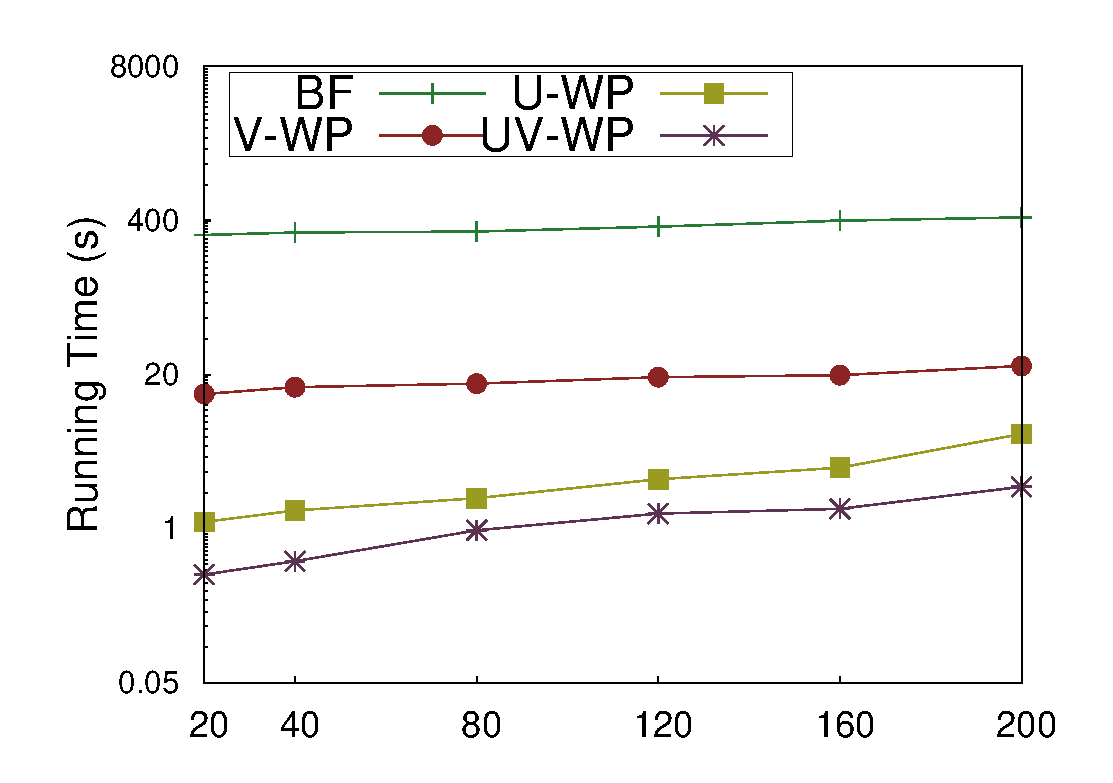
\includegraphics[width=\textwidth]{chapter4/exp/offline/varyp/stock_vary_p.eps}
        \caption{STOCK}
    \end{subfigure}
    \begin{subfigure}[b]{0.45\textwidth}
        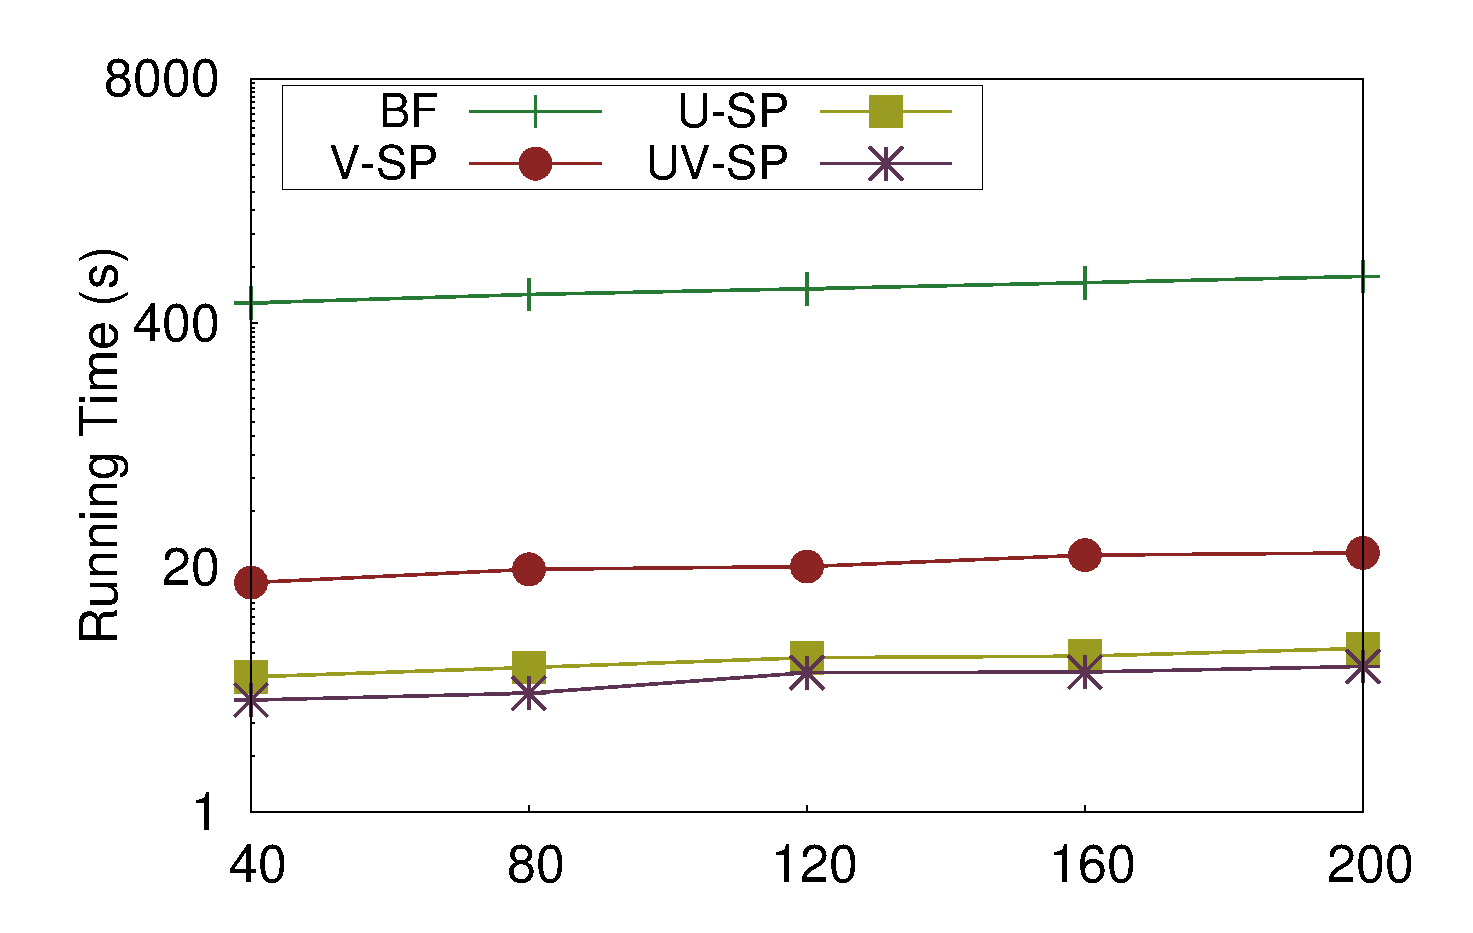
\includegraphics[width=\textwidth]{chapter4/exp/offline/varyp/pems_vary_p.eps}
        \caption{PEMS}
    \end{subfigure}
\caption{Ranked-streak generation in the offline scenario with varying $p$.}
\label{exp:offline_performance_vary_p}
\end{figure}

%\subsubsection{Candidate theme generation with varying $h$}
%We then study the performance of four algorithms wrt. the number of events and report the results 
%in Fig.~\ref{exp:offline_performance_vary_n}. As presented in the figures, when $h$ increases, 
%the running time for all the four algorithms also increases. This is because more event windows need to be evaluated. 
%Again, pruning-based methods are much efficient than the baseline method. When both pruning methods are adapted, our method obtains hundreds of times faster than the baseline method.
\subsubsection{Ranked-Streak Generation varying $h$}
We then study the performance of the four algorithms with respect to the number of events and report the results 
in Figure~\ref{exp:offline_performance_vary_n}. As the figure shows, when $h$ increases, 
the running times for all four algorithms increase. This is because more streaks need to be evaluated. 
Again, pruning-based methods are much more efficient than the baseline method. When both pruning methods are adopted, our method (UV-SP) obtains hundreds of times faster than the baseline method.

%
%\subsubsection{Sketch discovery with varying $k$}
%After candidate themes are generated, we greedily find the $k$-sketch for each subject. 
%Here, we study the effect of $k$ on the performance of the greedy algorithm. The results on four datasets are presented in Table~\ref{exp:offline_greedy}. The table indicates that for all four datasets, as $k$ increases, the running time of the greedy algorithm proportionally increases. This is because the complexity of the greedy algorithm is $O(k\Sigma_s|\mathbb{N}_s|)$. Since PEMS is the largest dataset with highest $\Sigma_s|\mathbb{N}_s|$, greedy algorithm performs worst on PEMS. As we observe that, even greedy algorithm takes upto 400 seconds on PEMS, the performance of the exact solution with quadratic complexity is not acceptable. This confirms the necessity of adapting the approximation algorithm.

\subsubsection{Sketch Discovery varying $k$}
After ranked-streaks are generated, we greedily find the $k$-sketch for each subject. 
Here, we study the effect of $k$ on the performance of the greedy algorithm. The results on the four datasets are presented in Table~\ref{exp:offline_greedy}. The table indicates that the running time of the greedy algorithm 
increases proportionally to $k$.
%
% that for all four datasets, as $k$ increases, the running time of the greedy algorithm proportionally increases. 
This is because the complexity of the greedy algorithm is $O(k\Sigma_s|\mathbb{N}_s|)$. Since PEMS is the largest dataset with highest $\Sigma_s|\mathbb{N}_s|$, the greedy algorithm performs worst on PEMS. We also observe that the greedy algorithm takes near 500 seconds on PEMS, which implies that the performance of exact solutions with cubic complexity is not acceptable. This confirms the necessity of adopting the approximate algorithm.

\begin{figure}[t]
\centering
    \begin{subfigure}[b]{0.45\textwidth}
        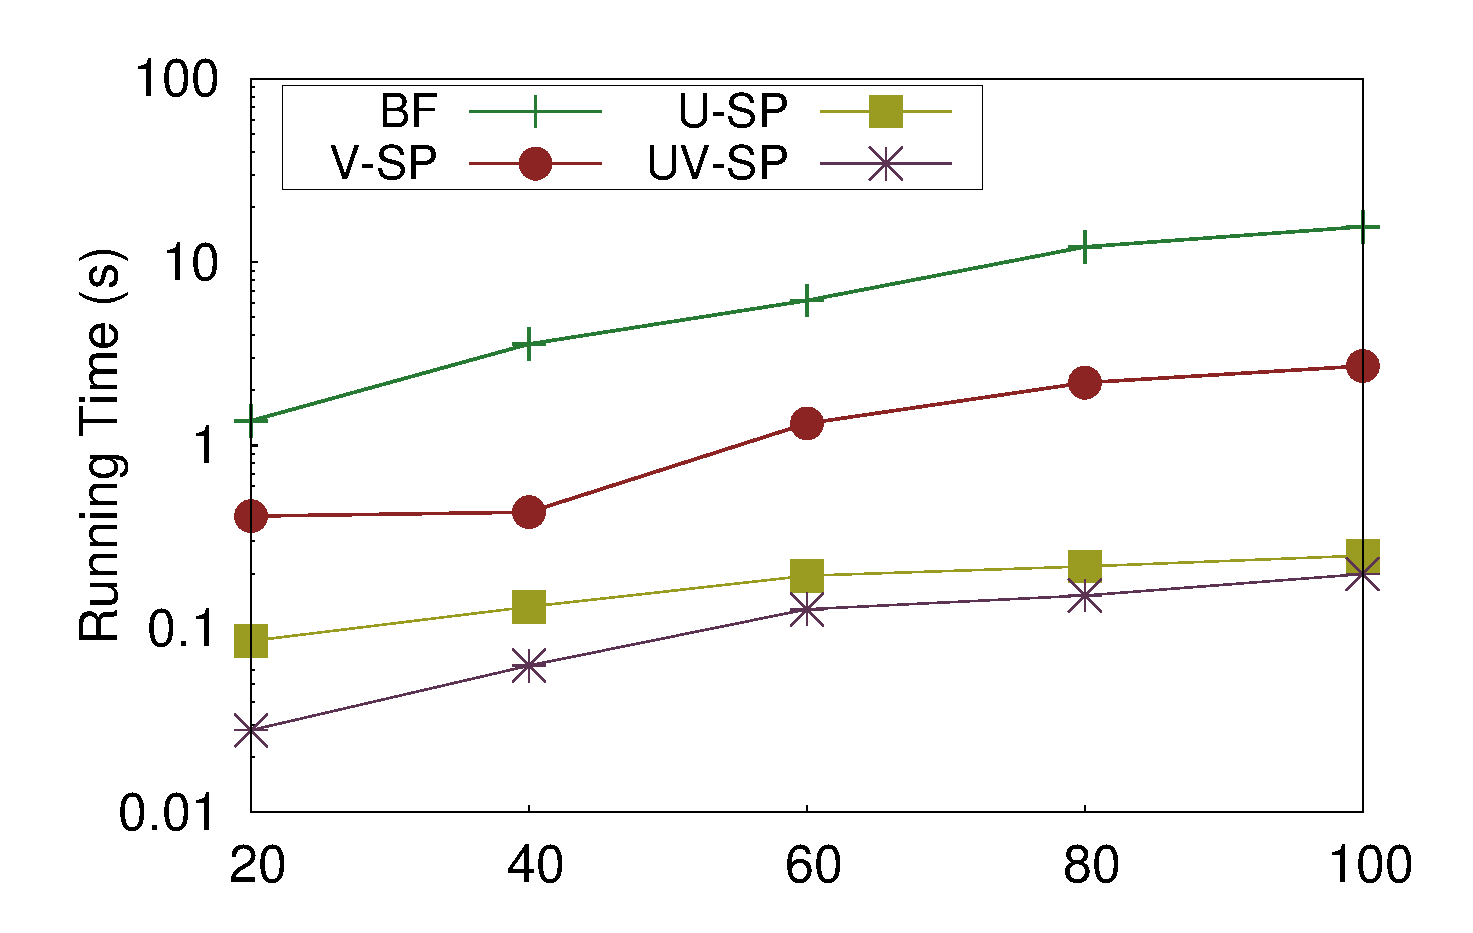
\includegraphics[width=\textwidth]{chapter4/exp/offline/varyh/nba_vary_h.eps}
        \caption{NBA}
    \end{subfigure}
    \begin{subfigure}[b]{0.45\textwidth}
        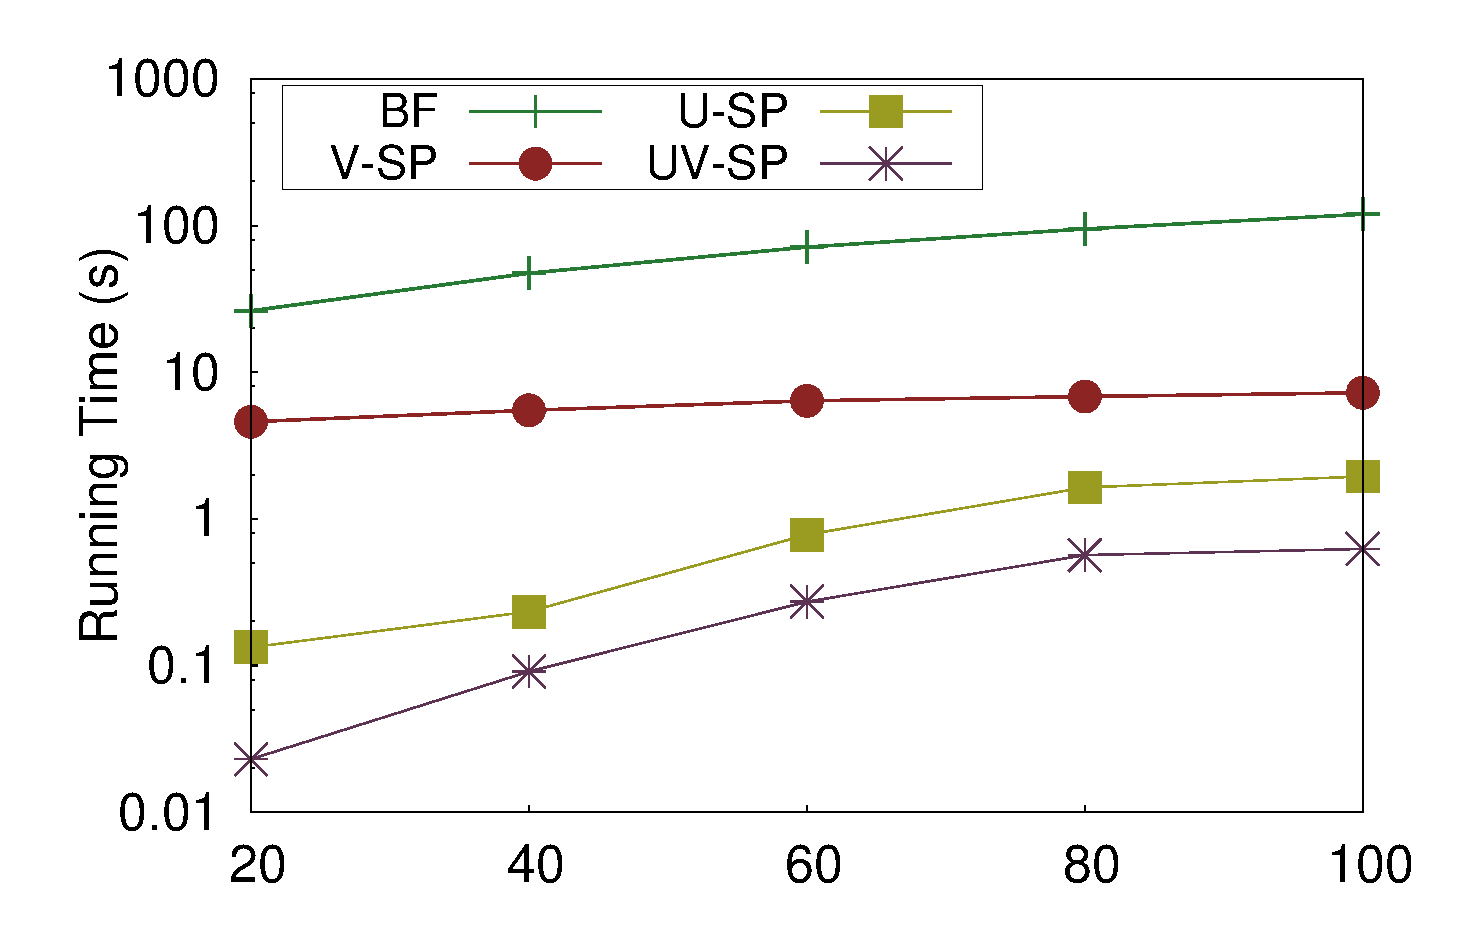
\includegraphics[width=\textwidth]{chapter4/exp/offline/varyh/power_vary_h.eps}
        \caption{POWER}
    \end{subfigure}
    \begin{subfigure}[b]{0.45\textwidth}
        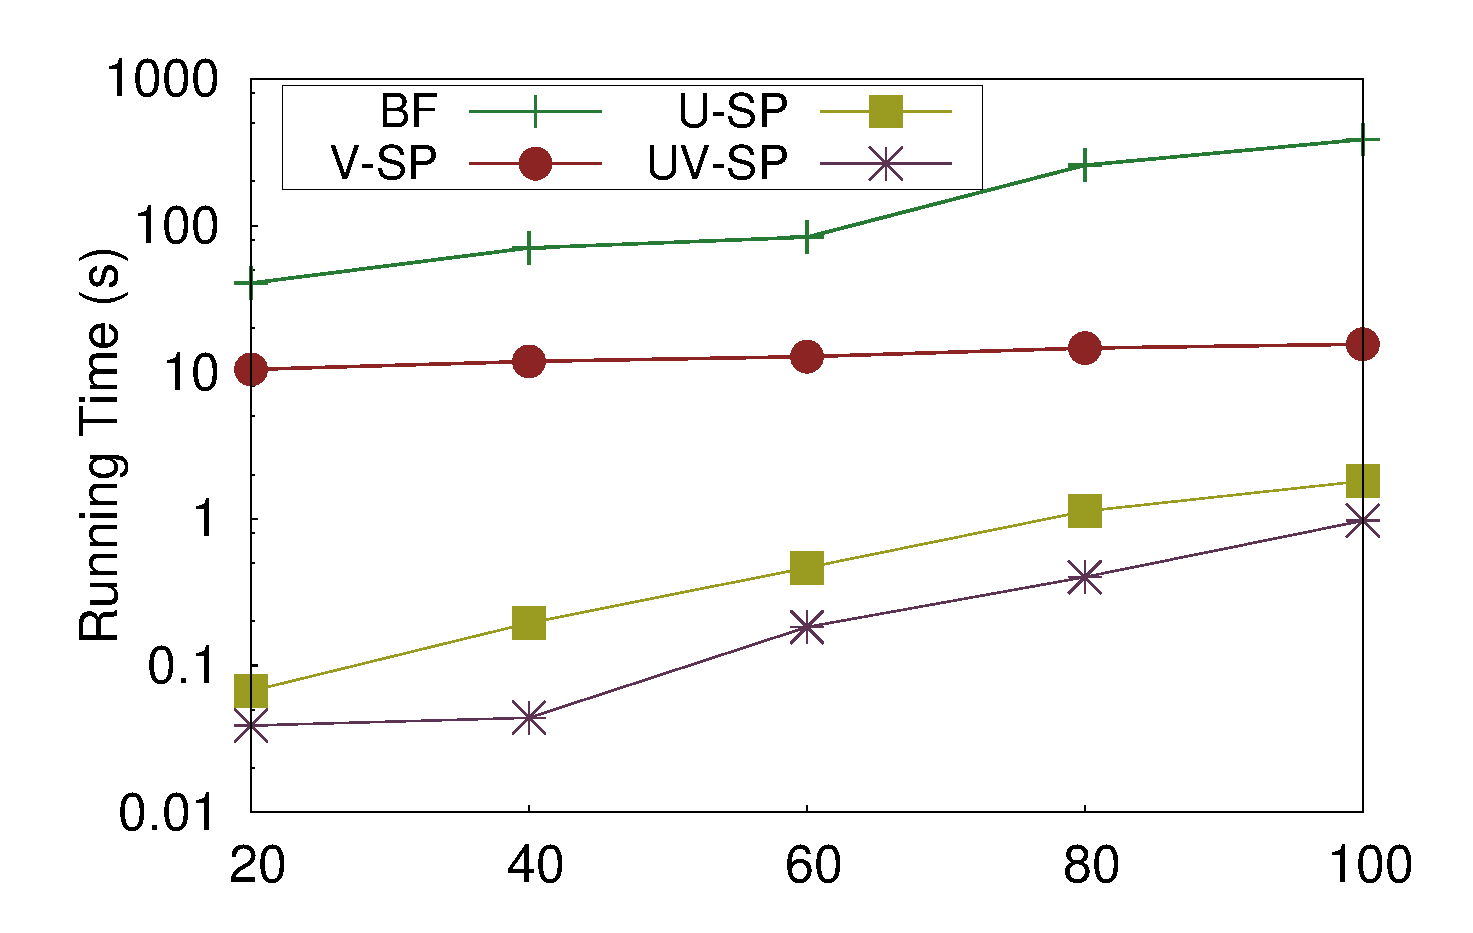
\includegraphics[width=\textwidth]{chapter4/exp/offline/varyh/stock_vary_h.eps}
        \caption{STOCK}
    \end{subfigure}
    \begin{subfigure}[b]{0.45\textwidth}
        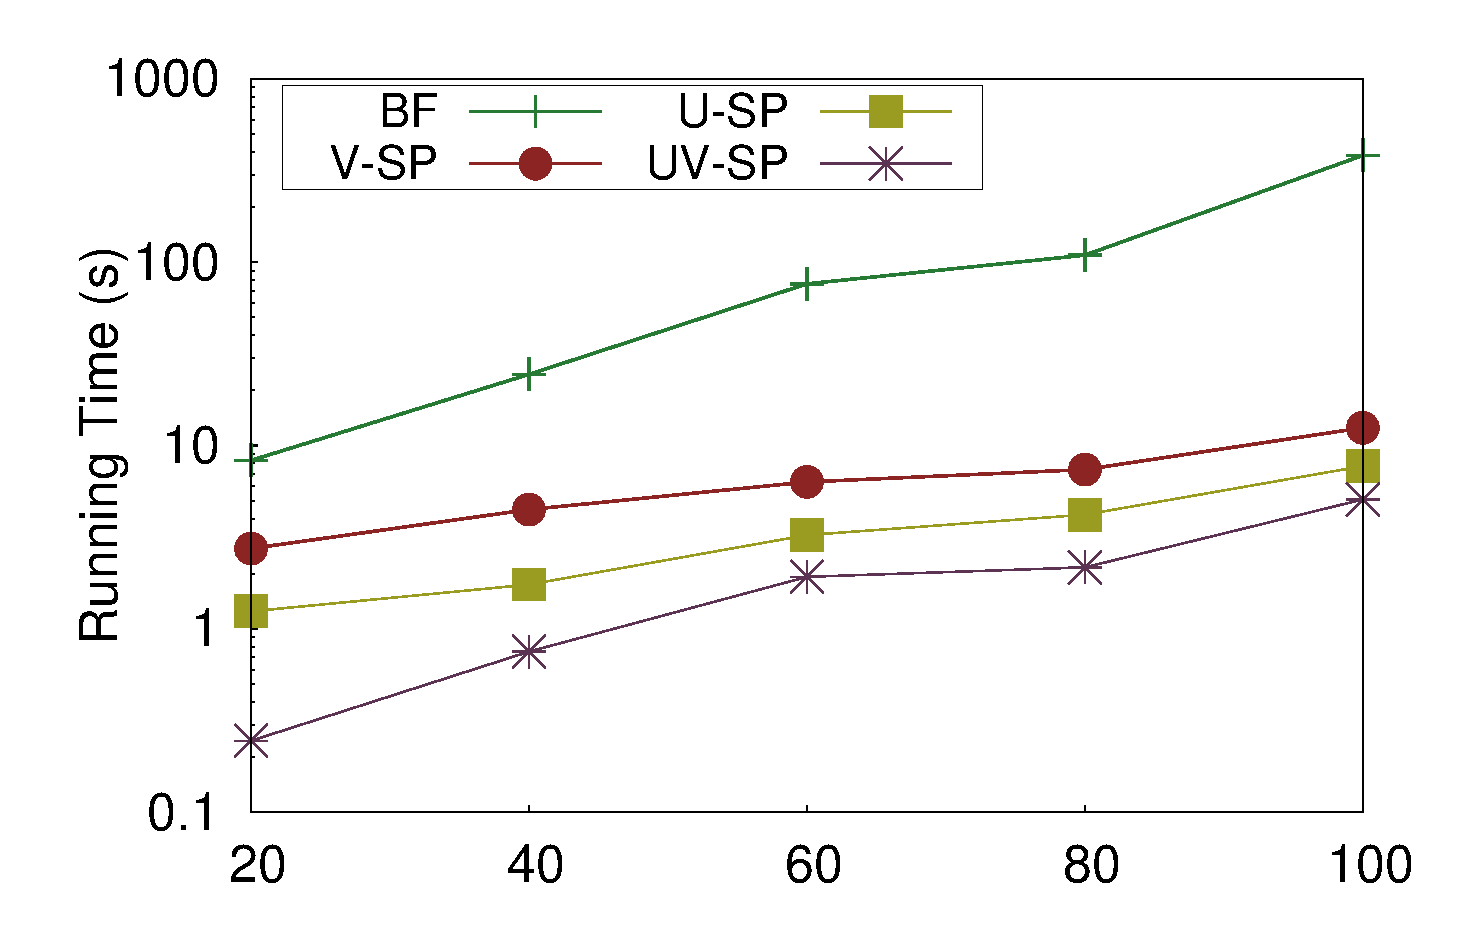
\includegraphics[width=\textwidth]{chapter4/exp/offline/varyh/pems_vary_h.eps}        
        \caption{PEMS}
    \end{subfigure}
\caption{Ranked-streak generation in the offline scenario with varying $h$.}
\label{exp:offline_performance_vary_n}
\end{figure}

%\begin{figure}[h]
%\centering
%        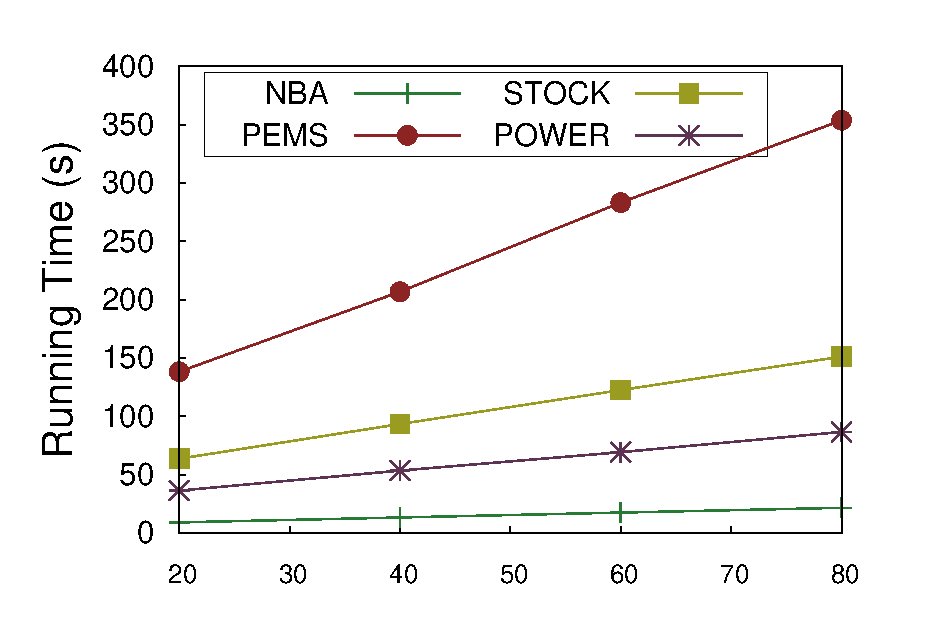
\includegraphics[width=0.25\textwidth]{offline/greedy/offline_varyk.eps}
%\caption{Greedy algorithm performance in offline sketch discovery with varying $k$}
%\label{exp:offline_greedy}
%\end{figure}


\begin{table}
\centering
\caption{Sketch discovery with varying $k$ in (ms)}\label{exp:offline_greedy}
\begin{tabular}{|c|c|c|c|c|c|}
\hline 
\textbf{k} & \textbf{20} & \textbf{40} & \textbf{60} & \textbf{80}& \textbf{100} \\ 
\hline 
NBA & 9,097 & 13,345	& 17,500	& 21,597 & 	30,769 \\ 
\hline 
POWER & 36,297 & 53,513 & 69,300 &	86,603 &	122,856
\\ 
\hline 
STOCK & 63,679	& 93,415 &	122,500 &	151,179 &	215,386\\ 
\hline 
PEMS & 138,224	& 206,820 &	283,190 &	353,766	& 491,000 \\ 
\hline 
\end{tabular} 
\end{table}




\subsection{Online Sketch Maintenance}
\label{subsec:exp-online}
In the online scenario, we evaluate the following four algorithms in our performance study:

%\noindent\textbf{Sketch Computing (SC)}: SC examines all event windows generated from a fresh event.  Whenever there is an update in any subject's sketch, Algorithm~\ref{algo:greedy} will be invoked. To improve efficiency, the updates are processed in a batch manner, i.e., multiple updates
%on the same subject will be batched and processed by calling Algorithm~\ref{algo:greedy} once.

\noindent\textbf{Sketch Computing (SC)}. SC examines all streaks generated from a fresh event.
Then Algorithm~\ref{algo:greedy} is invoked for each affected subject.
% Whenever there is an update in any subject's sketch, Algorithm~\ref{algo:greedy} will be invoked. 
To improve efficiency, the updates are processed in batches, i.e., multiple updates on the same subject will be batched and processed by calling Algorithm~\ref{algo:greedy} once.

\noindent\textbf{Sketch with Early Termination (SET)}. SET adopts \emph{online-streak} bound in Theorem~\ref{thm:online_bound} for early termination.

\noindent\textbf{Approx. Sketch (AS)}. AS is similar to \emph{SC} except that it only computes the approximate sketches. 

\noindent\textbf{Approx. Sketch with Early Termination (ASET)}. ASET computes the approximate sketches with early termination, as shown in Algorithm~\ref{algo:online_overview}.

In the online setting, we are more interested in evaluating the throughput of algorithms. We report the performance with respect to $p$, $k$ and $h$.

\subsubsection{Query Throughput varying $p$}
We increase $p$ from 10 to 200 and the throughput results are 
shown in Figure~\ref{exp:online_mining_vary_P}.
The figure demonstrates similar patterns for all four datasets. As $p$ increases, 
the throughput of the four algorithms drops.
%This is because as $p$ increases, the time to maintain the $p$ best candidate themes
%as well as to update the sketch increases.
This is because as $p$ increases, the time required to maintain the top-$p$ ranked-streaks
as well as to update the sketch increases.
However, algorithms adopting 
\emph{online-streak bound} have higher throughput than their counterparts. 
This is because with early termination,
% fewer candidate themes are generated. 
fewer streaks are generated. 
We can also see that $SC$ and $ASC$ run very slowly in the online setting. 
This is because they need to invoke Algorithm~\ref{algo:greedy} upon every update.
This confirms the necessity of our approximate method as $ASET$ achieves up to 500x speedup as compared to $SC$.

\begin{figure}[t]
\centering
    \begin{subfigure}[b]{0.45\textwidth}
        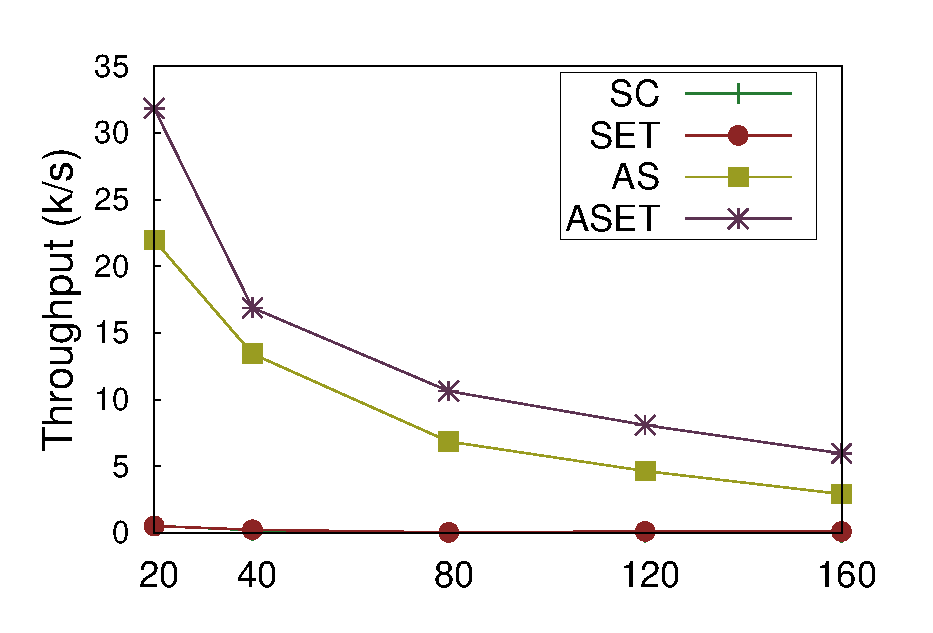
\includegraphics[width=\textwidth]{chapter4/exp/online/varyp/nba_varyp.eps}
        \caption{NBA}
    \end{subfigure}
    \begin{subfigure}[b]{0.45\textwidth}
        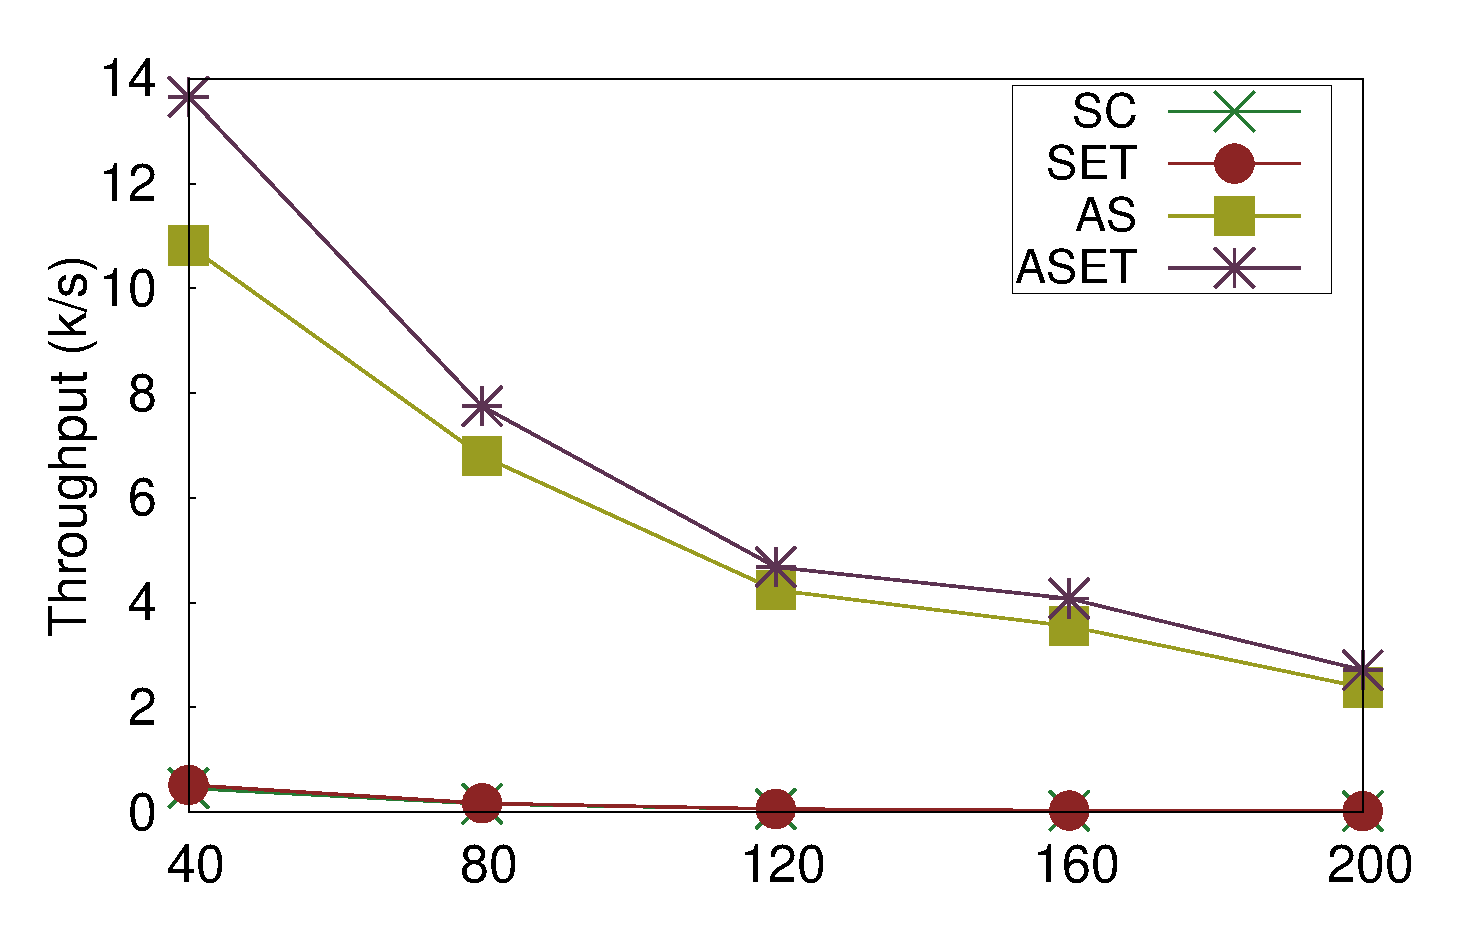
\includegraphics[width=\textwidth]{chapter4/exp/online/varyp/power_varyp.eps}
        \caption{POWER}
    \end{subfigure}
    \begin{subfigure}[b]{0.45\textwidth}
        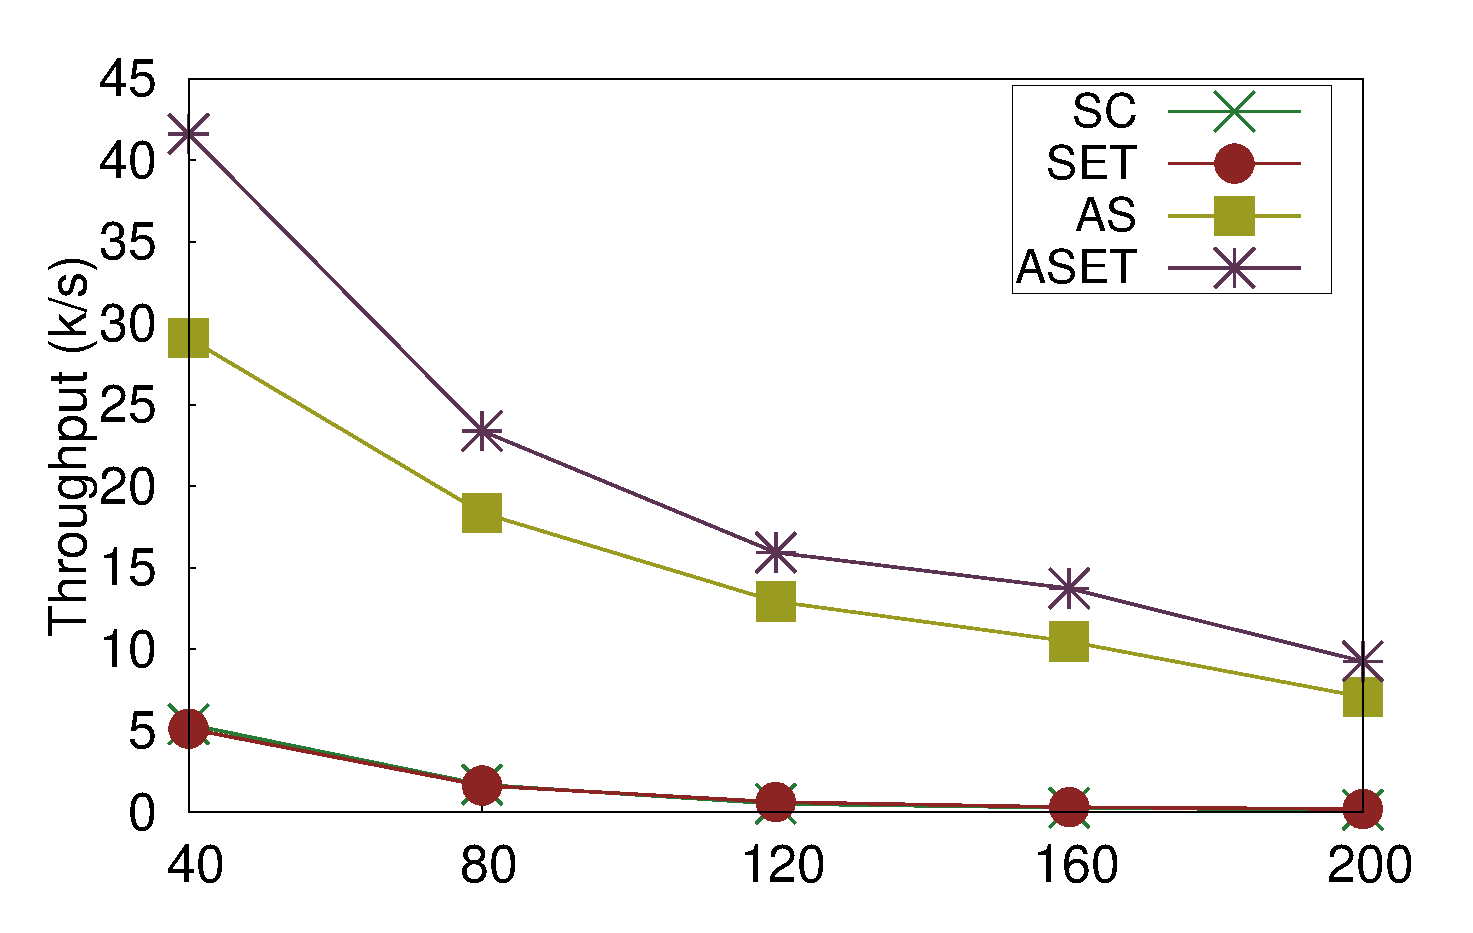
\includegraphics[width=\textwidth]{chapter4/exp/online/varyp/stock_varyp.eps}
        \caption{STOCK}
    \end{subfigure}
    \begin{subfigure}[b]{0.45\textwidth}
        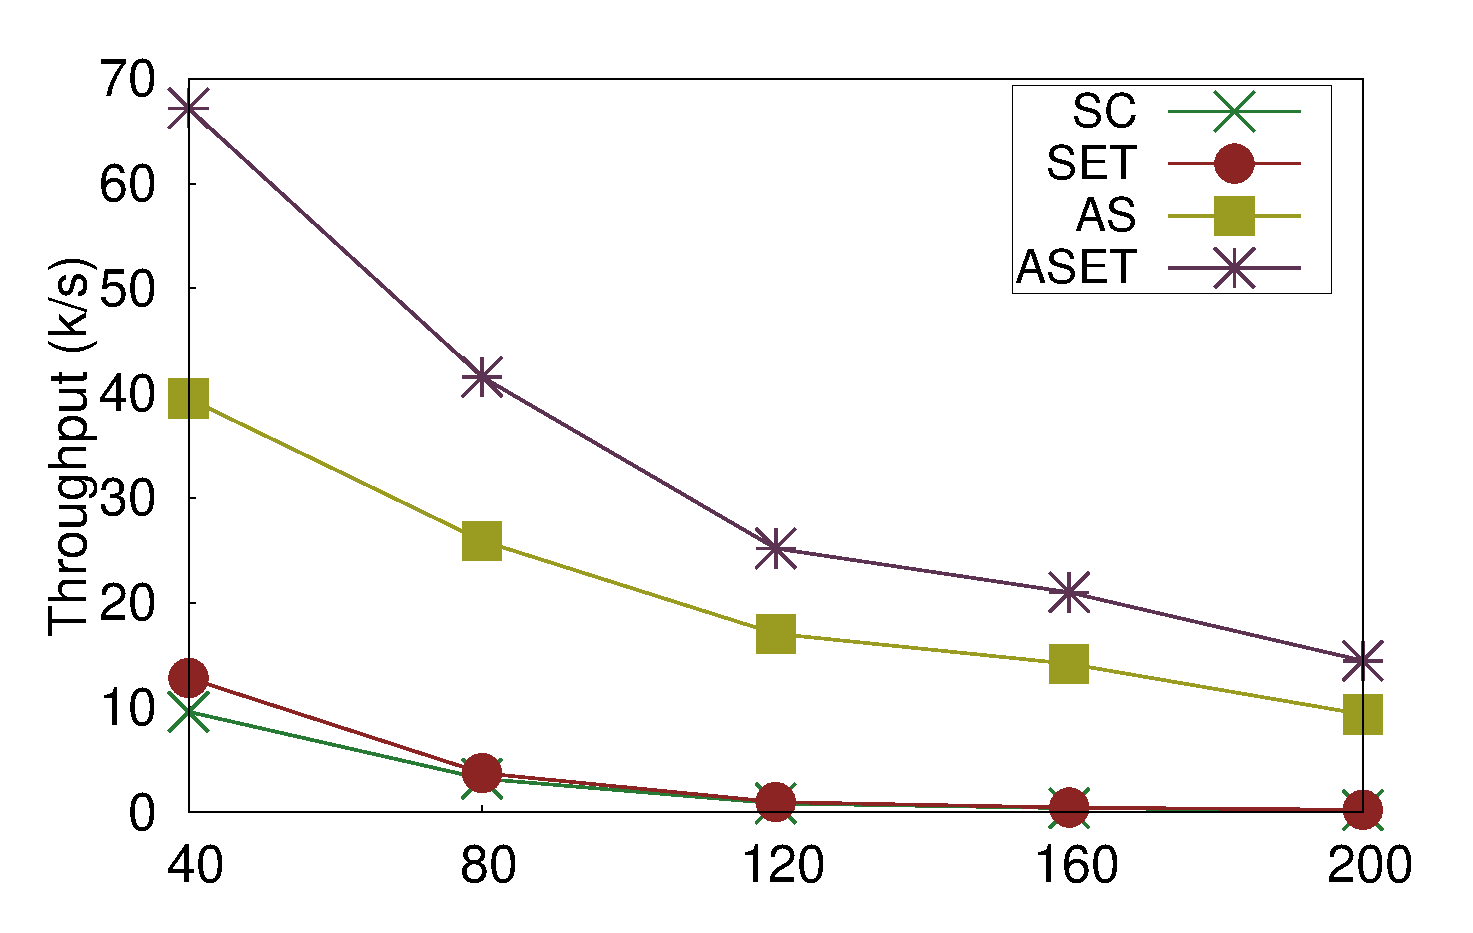
\includegraphics[width=\textwidth]{chapter4/exp/online/varyp/pems_varyp.eps}
        \caption{PEMS}
    \end{subfigure}
\caption{Throughput in online scenario with varying $p$.}
\label{exp:online_mining_vary_P}
\end{figure}

\subsubsection{Query Throughput varying $k$} 
We then evaluate how the throughput varies with respect to $k$. 
The results are presented in Figure~\ref{exp:online_mining_vary_k}.
The figure tells similar patterns as
Figure~\ref{exp:online_mining_vary_P}.
First, as $k$ increases, the throughput of all four algorithms decreases.
This is because as $k$ becomes larger, more operations are needed for maintaining the sketch.
Second, the throughput of $SC$ and $SET$ are an order of magnitude smaller than $AS$ and $ASET$.
This is because $SC$ and $SET$ repetitively call Algorithm~\ref{algo:greedy} which heavily depends 
on $k$.
%This is because of the repetitive calling of Algorithm~\ref{algo:greedy} for each arrival event,
%which heavily depends on $k$. 
We observe that in some datasets (e.g., Figure~\ref{exp:online_mining_vary_k} (a)) there is 100x boost for $ASET$ as compared to $SC$.

\begin{figure}[t]
\centering
    \begin{subfigure}[b]{0.45\textwidth}
        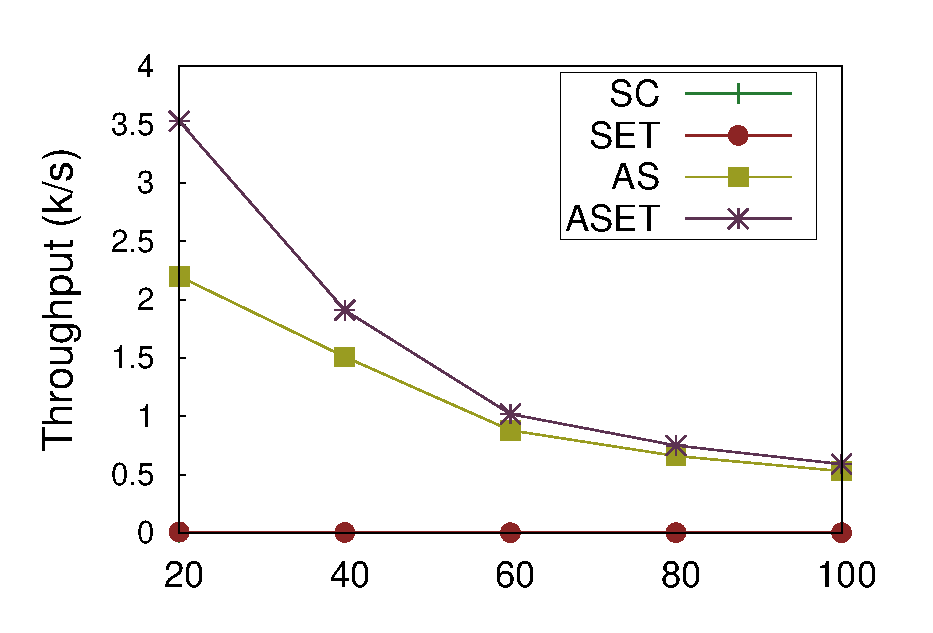
\includegraphics[width=\textwidth]{chapter4/exp/online/varyk/nba_varyk.eps}
        \caption{NBA}
    \end{subfigure}
    \begin{subfigure}[b]{0.45\textwidth}
        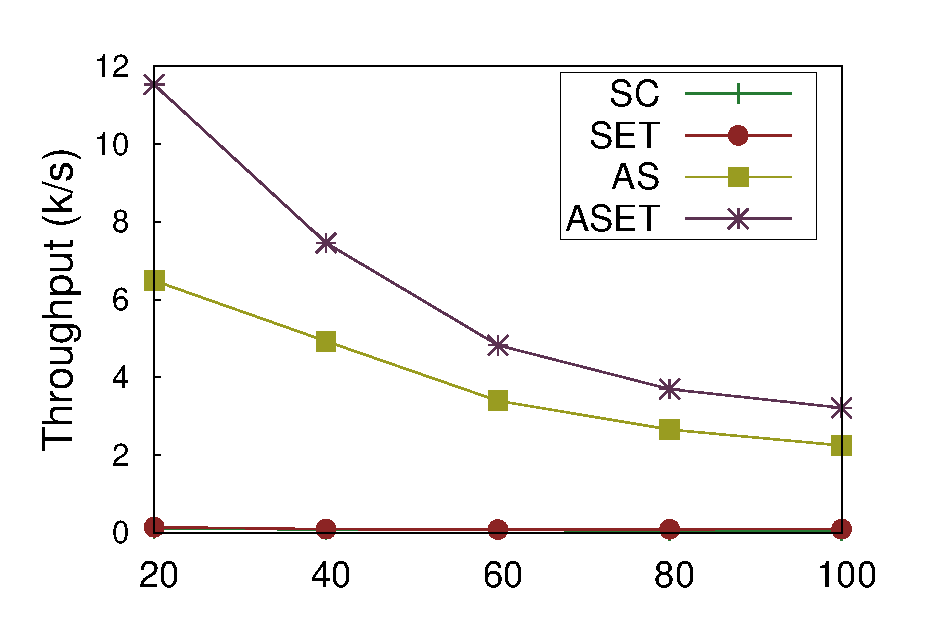
\includegraphics[width=\textwidth]{chapter4/exp/online/varyk/power_varyk.eps}
        \caption{POWER}
    \end{subfigure}
    \begin{subfigure}[b]{0.45\textwidth}
        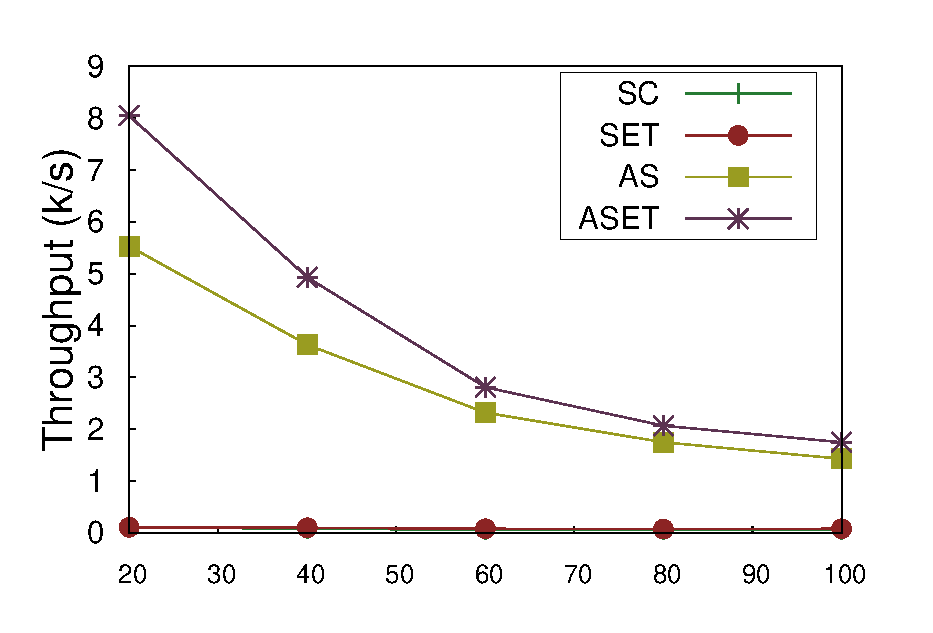
\includegraphics[width=\textwidth]{chapter4/exp/online/varyk/stock_varyk.eps}
        \caption{STOCK}
    \end{subfigure}
    \begin{subfigure}[b]{0.45\textwidth}
        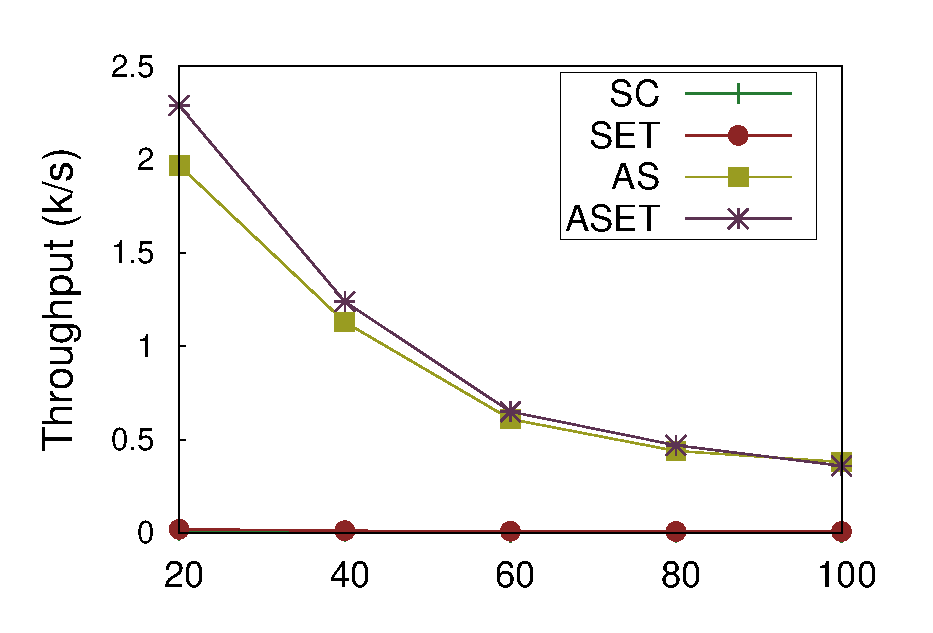
\includegraphics[width=\textwidth]{chapter4/exp/online/varyk/pems_varyk.eps}
        \caption{PEMS}
    \end{subfigure}
\caption{Throughput in the online scenario with varying $k$.}
\label{exp:online_mining_vary_k}
\end{figure}

\subsubsection{Query Throughput varying $h$}
Finally, we study the effect of $h$ in affecting the throughput.
We change $h$ from 20 to 100, and the results are represented in Figure~\ref{exp:online_mining_vary_h}.
As shown in the figure, when $h$ increases, 
the throughput of the four algorithms drops steadily.
This is because as $h$ increases, $|\mathbb{H}_s|$ for each subject
increases. Therefore in Algorithm~\ref{algo:online_overview}, more time is needed 
to process each streak. We notice that \emph{ASET} has a flatter slope than \emph{AS}; this
is benefit from the prunings of \emph{online-streak} bound.
\begin{figure}[h]
\centering
    \begin{subfigure}[b]{0.45\textwidth}
        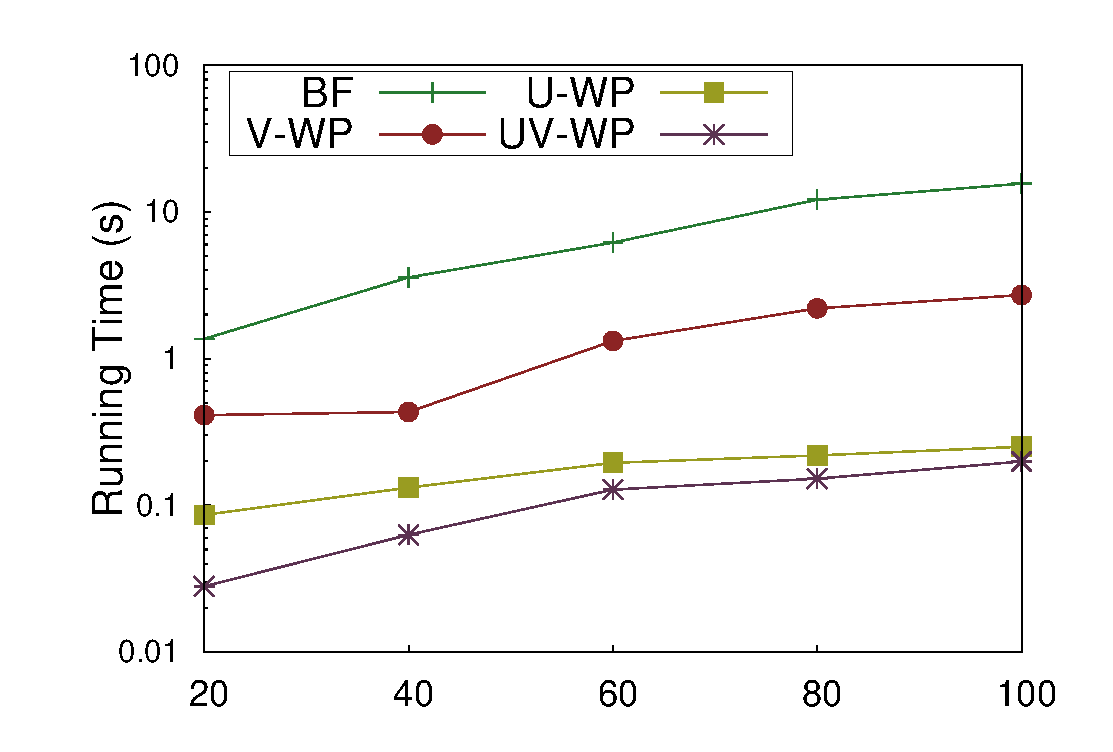
\includegraphics[width=\textwidth]{chapter4/exp/online/varyh/nba_varyh.eps}
        \caption{NBA}
    \end{subfigure}
    \begin{subfigure}[b]{0.45\textwidth}
        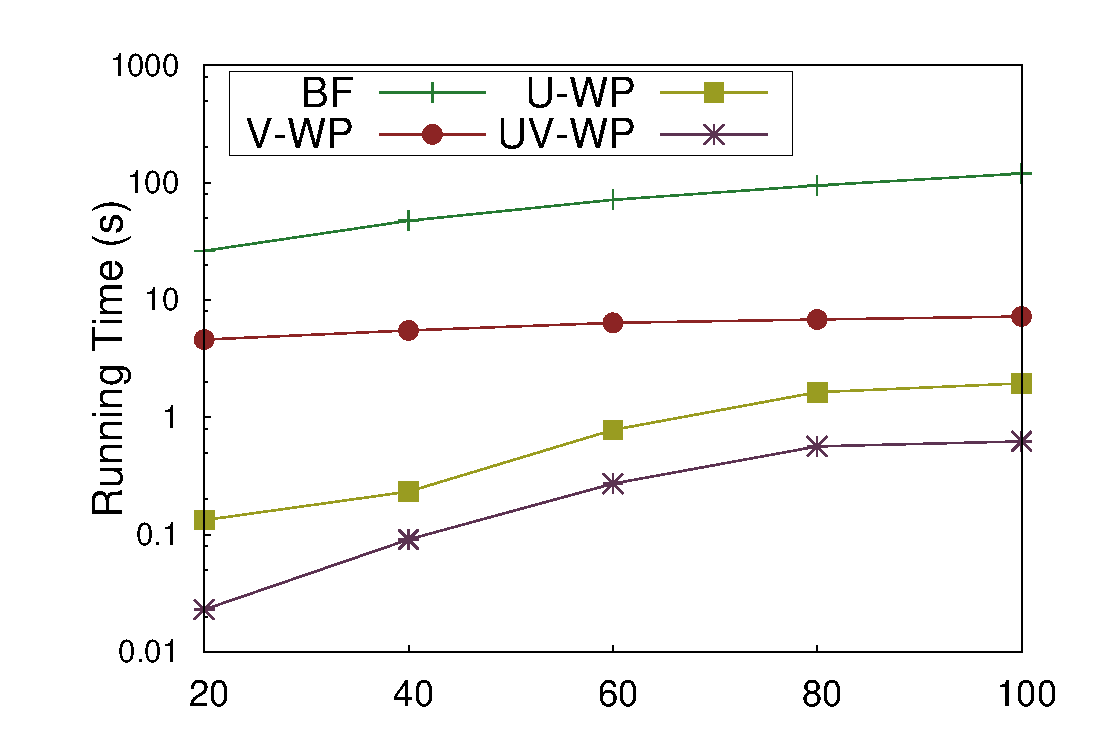
\includegraphics[width=\textwidth]{chapter4/exp/online/varyh/power_varyh.eps}
        \caption{POWER}
    \end{subfigure}
    \begin{subfigure}[b]{0.45\textwidth}
        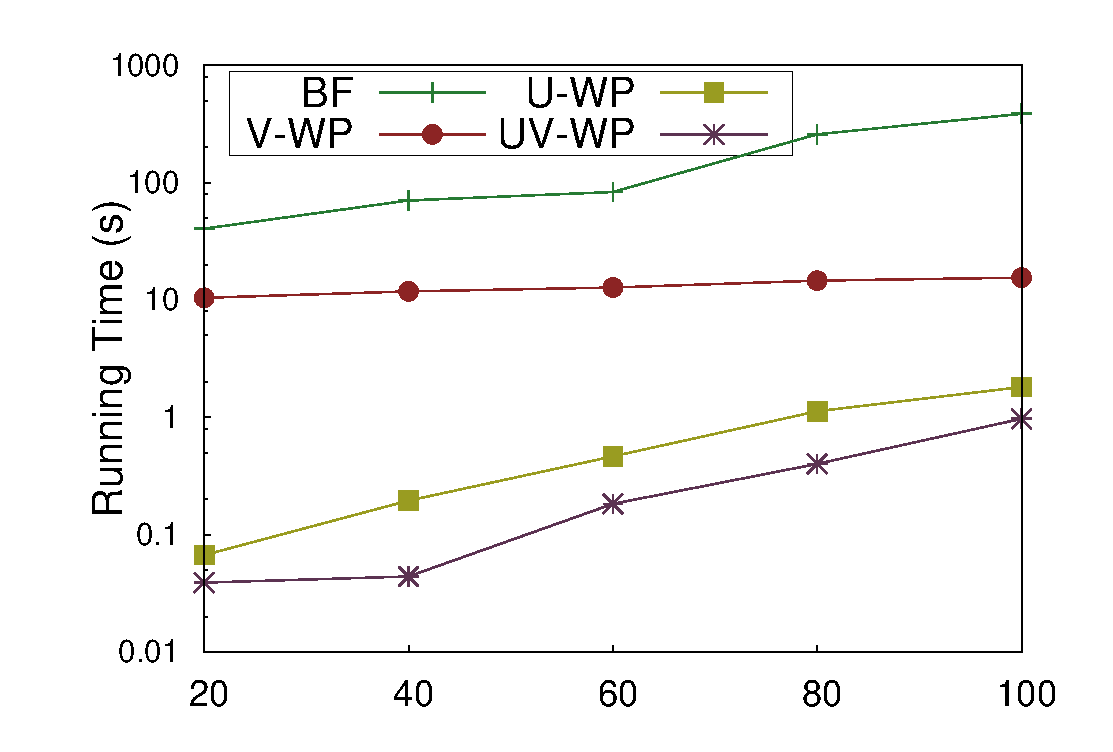
\includegraphics[width=\textwidth]{chapter4/exp/online/varyh/stock_varyh.eps}
        \caption{STOCK}
    \end{subfigure}
    \begin{subfigure}[b]{0.45\textwidth}
        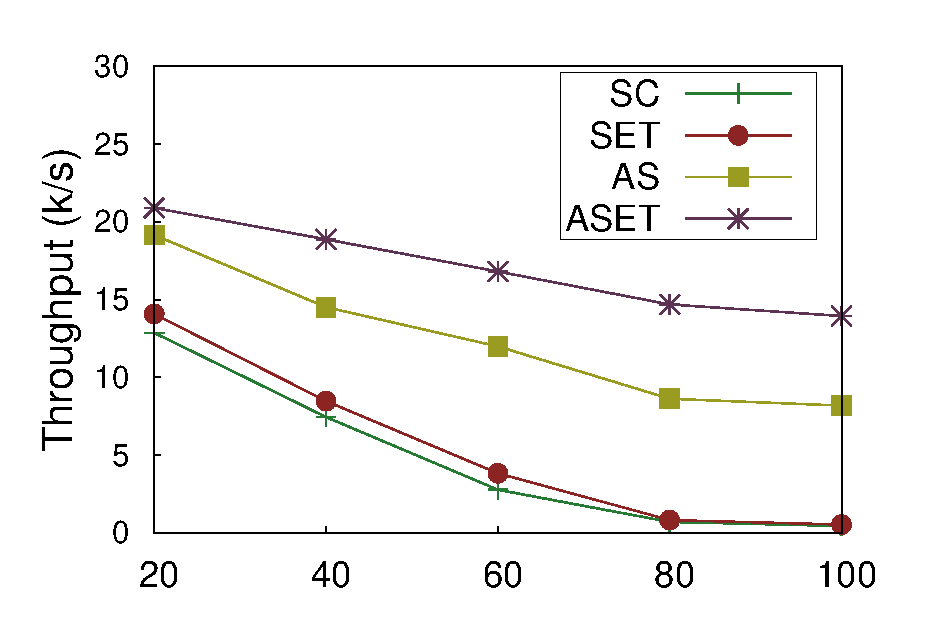
\includegraphics[width=\textwidth]{chapter4/exp/online/varyh/pems_varyh.eps}
        \caption{PEMS}
    \end{subfigure}
\caption{Throughput in the online scenario with varying $h$.}
\label{exp:online_mining_vary_h}
\end{figure}

\subsection{Comparison with Other Techniques}
\label{subsec:exp-survey}
We also compare the efficiency and effectiveness of our $k$-Sketch query with
the state-of-the-art Prominent Streaks query~\cite{zhang2014discovering} (denoted by the skyline method) in 
providing newsworthy summaries.

To study the efficiency, we implement the skyline algorithms as described in~\cite{zhang2014discovering} for
both online and offline scenarios. 
The results under all four datasets are presented in Figure~\ref{exp:sky_comp}. 
The figure demonstrates the superiority of our schemes in both scenarios.
%As the figure tells, our schemes outperform the skyline approaches in both 
%scenarios. 
Specifically, our offline scheme saves 63\% to 75\% processing time and our online scheme 
achieves 2 to 10 time throughput speedups. 
These results further indicate the efficiency of our schemes.
%$k$-Sketch query discovery solutions.
%Note that, it is computationally expensive to compute the ``rank'' information for prominent streaks. 


%we first modify the skyline technique in~\cite{zhang2014discovering} to consider ranks. In the offline scenario, the rank is computed using BF method, while in the online scenario, we directly keep the $WI$ and the rank can be easily maintained. We use the default parameters settings for both scenarios. Figs.~\ref{exp:sky_comp} (a)(b) show the running time comparisons under all four datasets. We can see that, when trying to adapt for rank-awareness, naively computing the rank on skyline method incurs high overheads. For instance, as presented in Fig.~\ref{exp:sky_comp} (a), in the offline scenario, the running time of skyline method is order of magnitude slower than sketch method. This supports the use of pruning techniques in computing the ranks. Similarly, as shown in Fig.~\ref{exp:sky_comp} (b), in the online scenario, our sketch method still has a much better throughput. Although skyline method is free from passive update, as it is computationally expensive to maintain online skyline points, we still observe an upto 5 times boosts of sketch method.

%We also compare both the performance and effectiveness of our sketch discovery with prominent streak
%technique~\cite{zhang2014discovering} (denoted by skyline method). Due to the mismatched goal of sketch and skyline, these experiments only serve as references.
%
%To study the efficiency, we first modify the skyline technique in~\cite{zhang2014discovering} to consider ranks. In the offline scenario, the rank is computed using BF method, while in the online scenario, we directly keep the $WI$ and the rank can be easily maintained. We use the default parameters settings for both scenarios. Figs.~\ref{exp:sky_comp} (a)(b) show the running time comparisons under all four datasets. We can see that, when trying to adapt for rank-awareness, naively computing the rank on skyline method incurs high overheads. For instance, as presented in Fig.~\ref{exp:sky_comp} (a), in the offline scenario, the running time of skyline method is order of magnitude slower than sketch method. This supports the use of pruning techniques in computing the ranks. Similarly, as shown in Fig.~\ref{exp:sky_comp} (b), in the online scenario, our sketch method still has a much better throughput. Although skyline method is free from passive update, as it is computationally expensive to maintain online skyline points, we still observe an upto 5 times boosts of sketch method.

To study the effectiveness, we conduct a user study over Amazon Mechanical Turk\footnote{https://requester.mturk.com} to evaluate the attractiveness of the summaries generated by different methods. For our method, we set $\alpha=0.5$ to pay equal attention to the strikingness and the coverage. For the skyline method, due to the overwhelming skylines generated for each subject, 
%we propose three augmented methods to pick $k$ of them. In total, we have the following five algorithms to compare with:
we propose two augmented methods to pick $k$ of them. In total, we compare the following four algorithms:
% In total, we have the following four algorithms to compare with:
\begin{enumerate}
\item{$SK$: selects the $k$-sketch for each player generated by the offline $k$-Sketch query.}
\item{$SK_a$: selects the $k$-sketch for each player generated by the online $k$-Sketch query.}
\item{$SY_m$: randomly selects $k$ streaks for each player from the bunch of skylines generated by~\cite{zhang2014discovering}.}
%\item{$SY_m$: selects $k$ streaks sorted by freshness of the events;}
%\item{$SY_r$: selects $k$ rank-attached streaks sorted by the scoring function proposed in this paper;}
\item{$SY_r$: attaches ranks\footnote{Rank is generated by our offline method} to the streaks in $SY_m$.}
\end{enumerate}

We then apply each method on the NBA dataset and set $k=5$ to generate $5$ streaks 
for each player. 
Each streak is then translated into a news theme in the following format:
%In our experimental setting, we use the NBA dataset and set $k=20$ to generate $20$ news themes for each player. Each news theme is in the following format:

\textit{2003/04/14: Jordan obtained 30.3 PPGA\footnote{PPGA:Point-per-game-average} in 989 straight games, ranked $1^{st}$ in NBA history!!}

%Thus, the four methods generate four summaries for a player.
%Thus, each algorithm results in  $4$ summaries for a player.
We design each job in AMT to contain $5$ questions and each question
presents the four summaries of a player generated by the four methods. 
A sample question regarding ``Kobe Bryant''
is listed in Table~\ref{tbl:survey-case}. 
Due to space limitation, we present $SY_m$ and $SY_r$ in one row, since they
essentially report the same streak, except that $SY_r$ provides additional rank information.
% for the same random player. 
%Each question presents the $5$ news themes generated by one algorithm. 
We then ask the respondents to endorse each summary based on the level of attractiveness.
We receive responses from 100 participants who have knowledge in 
NBA\footnote{In AMT, we are able to request respondents with 
certain qualifications, i.e. knowledgeable in NBA.}. 
Then, for each algorithm, we count the frequency of it being endorsed as the best
and report the percentage results in the pie chart in Figure~\ref{exp:survey}. 

The chart clearly shows that $SK$ is the most effective method as
it takes $51\%$ of the endorsements from the respondents. Overall,
Sketch based methods (i.e., $SK$ and $SK_a$) receive $75\%$ endorsements,
which win the skyline methods (i.e., $SY_m$ and $SY_r$) by three times.
The chart also shows that, when applied with the rank information (i.e., $SY_r$),
the number of endorsements increases dramatically,
more than two times of the original number of endorsements (i.e., $SY_m$).
This also implies the effectiveness of our ranked-streaks.
We can also observe the quality differences of the four methods in Table~\ref{tbl:survey-case}. 
As the table shows, $SY_m$ and $SY_r$ output
streaks concentrating on a shorter period (i.e., 2006) as compared
with the output of $SK_a$ and $SK$ (i.e., 2003-2008).
This is because Kobe unprecedentedly scored 81 points on 2006/01/22, thus most skylines
are associated with that event.
Moreover,
the streaks selected by $SY_m$ and $SY_r$ are not ranked well as compared with
the results of $SK_a$ and $SK$. The reason is that skyline based methods only
consider the local prominence (i.e., non-dominated in one's career) but $k$-Sketch considers
the global prominence (i.e., rank in history).

 


%Meanwhile, its approximate variant $SK_a$ in the online scenario also achieved good performance and ranked as the second most attractive.
%Without any ranking, the skyline streak method~\cite{zhang2014discovering} gets the worst performance. We observe that there are still near 20\% responses pick skyline streaks as top-interesting. This is because the news themes generated by sketch and skyline have overlaps. For example, the news ``Michael Jordan has an average points of 30.30 for 989 games'' appears in the theme results of all five algorithms. In fact, we notice 24\% overlapped event windows between sketch and skyline methods. Under such circumstances, users may choose at random, which explains the 20\% responses for skyline streaks.
%The ranking based on freshness can slightly improve the attractiveness. However, when applied with our proposed ranking function, the number of users preferring the ranked skyline results increases dramatically, nearly two times of the original number of users. This also implies the effectiveness of our scoring function.

\begin{figure}[t]
\centering
    \begin{subfigure}[b]{0.45\textwidth}
        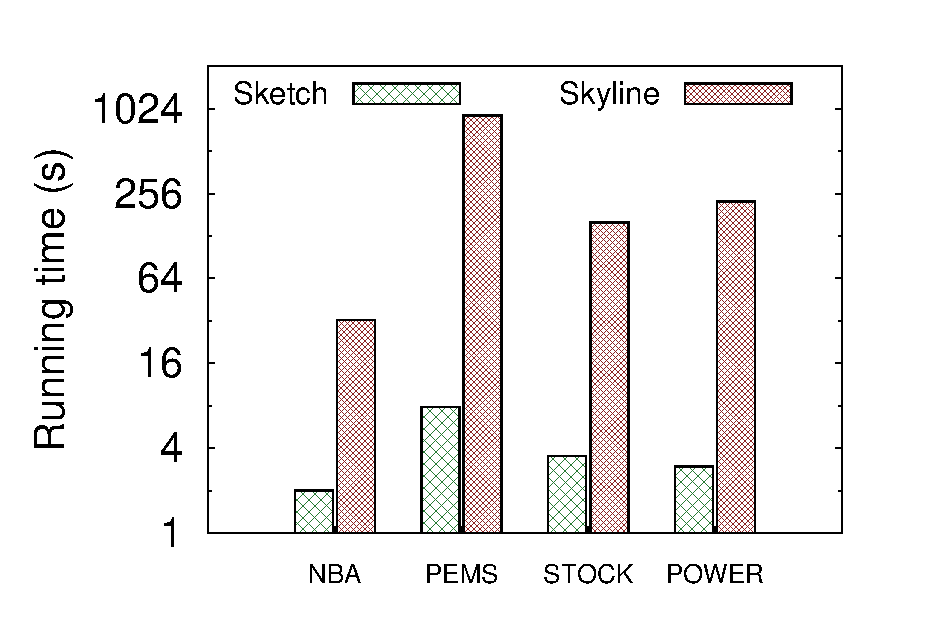
\includegraphics[width=\textwidth]{chapter4/exp/sky_comp/sky_comp_offline.eps}
        \caption{Offline Scenario}
    \end{subfigure}
    \begin{subfigure}[b]{0.45\textwidth}
        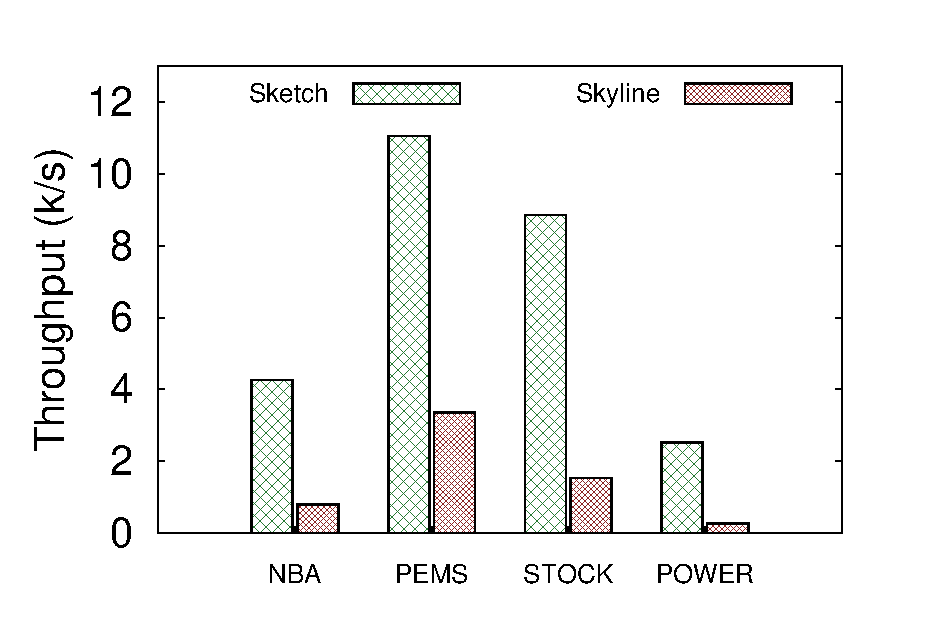
\includegraphics[width=\textwidth]{chapter4/exp/sky_comp/sky_comp_online.eps}
        \caption{Online Scenario}
    \end{subfigure}
\caption{Efficiency comparison with prominent streaks.}
\label{exp:sky_comp}
\end{figure}

\begin{figure}[h]
\centering
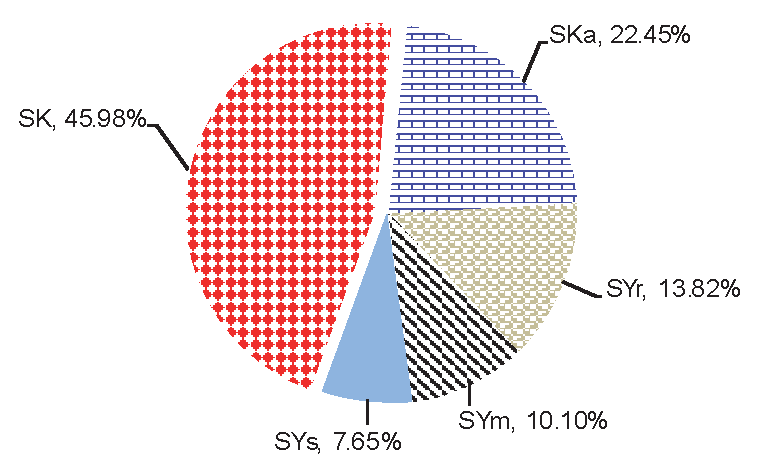
\includegraphics[width=0.8\textwidth]{chapter4/exp/survey/survey.eps}
\caption{Percentage of endorsements received as the most attractive.}
\label{exp:survey}
\end{figure}

\begin{table}
\caption{Summaries of ``Kobe Bryant'' on Point-per-game-average (PPGA) obtained by the four methods. $SY_r$ corresponds
to the same $SY_m$ streak with augmented rank information.}
\label{tbl:survey-case}
\centering
\begin{tabular}{|l|p{12cm}|}
\hline
\textbf{Method}          & \textbf{Career Summaries Generated                                                                                             } \\ \hline
\multirow{5}{0.5cm}{$SY_m$ ($SY_r$)} &1. \textbf{2006/04/16}, Kobe obtained \textbf{37.05} PPGA in \textbf{57} straight games (ranked \textbf{10} in NBA history)!    \\ %\cline{2-2}
						 &2. \textbf{2006/04/16}, Kobe obtained \textbf{35.09} PPGA in \textbf{85} straight games (ranked \textbf{111} in NBA history)!  \\ %\cline{2-2} 
                         &3. \textbf{2006/04/19}, Kobe obtained \textbf{36.91} PPGA in \textbf{61} straight games (ranked \textbf{12} in NBA history)!   \\ %\cline{2-2}
                         &4. \textbf{2006/11/03}, Kobe obtained \textbf{35.85} PPGA in \textbf{75} straight games (ranked \textbf{63} in NBA history)!  \\ %\cline{2-2}
                         &5. \textbf{2006/11/08}, Kobe obtained \textbf{35.29} PPGA in \textbf{78} straight games (ranked \textbf{85} in NBA history)!  
\\ \hline
\multirow{5}{0.5cm}{$SK_a$}  &1. \textbf{2003/03/11}, Kobe obtained \textbf{38.05} PPGA in \textbf{20} straight games, ranked \textbf{25} in NBA history! \\ %\cline{2-2}
                         &2. \textbf{2006/02/08}, Kobe obtained \textbf{38.67} PPGA in \textbf{28} straight games, ranked \textbf{1} in NBA history!    \\ %\cline{2-2}
                         &3. \textbf{2006/02/26}, Kobe obtained \textbf{38.10} PPGA in \textbf{30} straight games, ranked \textbf{1} in NBA history! \\ %\cline{2-2}
                         &4. \textbf{2006/04/19}, Kobe obtained \textbf{37.17} PPGA in \textbf{56} straight games, ranked \textbf{5} in NBA history!  \\ %\cline{2-2}
                         &5. \textbf{2007/10/30}, Kobe obtained \textbf{32.27} PPGA in \textbf{212} straight games, ranked \textbf{194} in NBA history!                  				 					 
\\ \hline
\multirow{5}{0.5cm}{$SK$}  &1. \textbf{2003/02/21}, Kobe obtained \textbf{43.20} PPGA in \textbf{10} straight games, ranked \textbf{3} in NBA history!    \\ %\cline{2-2}
                         &2. \textbf{2006/01/22}, Kobe obtained \textbf{81.00} PPGA in \textbf{1} straight games, ranked \textbf{1} in NBA history!     \\ %\cline{2-2}
                      	 &3. \textbf{2006/02/11}, Kobe obtained \textbf{38.24} PPGA in \textbf{29} straight games, ranked \textbf{1} in NBA history! \\ %\cline{2-2}
                         &4. \textbf{2007/03/30}, Kobe obtained \textbf{46.12} PPGA in \textbf{8} straight games, ranked \textbf{1} in NBA history!     
\\ %\cline{2-2}
					&5. \textbf{2008/02/01}, Kobe obtained \textbf{32.24} PPGA in \textbf{216} straight games, ranked \textbf{195} in NBA history!
\\\hline
\end{tabular}

\end{table}

\subsection{Case Study on Real Data}
We further study the $k$-Sketch query in the NBA dataset.
We compute a $5$-sketch for the player ``Dominique-Wilkins'' using different $\alpha$
and list the ranked-streaks in Table~\ref{tbl:real-alpha}. 
As the table shows, when $\alpha$ is small (i.e., $0.1$), 
the streaks selected tend to have higher ranks.
On the other hand, when $\alpha$ is large (i.e., $0.9$), the streaks have larger coverage.

We observe several interesting facts from the sketches. 
First, the streaks with highest coverage (i.e., $\alpha = 0.9$)
concentrate in the period 1986-1993, while the highest ranked-streaks (i.e., $\alpha = 0.1$) locate in the period 1986-1988. Looking
up the ground truth\footnote{\url{http://www.nba.com/history/players/wilkins_stats.html}}, 
we find that ``Dominique'''s prime career is in 1985-1993 and he was selected
into the All-Star team every year in 1986-1988, which is consistent with our discoveries.
Second, our $k$-Sketch query also discovers a length-1 streak of 57 points (in 1986-04-10, ranked $11^{th}$ in history), 
which is in fact the career-highest points scored by ``Dominique''\footnote{\url{http://articles.latimes.com/1986-12-11/sports/sp-2180_1_22-point-deficit}}.
Last, we notice that ``Dominique'' has a length-2 streak with an average score of 50 points, which ranks $8^{th}$ in history. 
Although this streak ranks better than the length-1 streak with 57 points, 
interestingly, it has not been reported in any news. This indicates that our $k$-Sketch query is able 
to discover interesting facts where human experts may miss.

\begin{table}[h]
\center
\caption{$5$-Sketches for ``Dominique-Wilkins'' from NBA dataset with respect to $\alpha$.}
\label{tbl:real-alpha}
\begin{tabular}{|l|c|c|c|c|}
\hline
\multirow{2}{*}{$\alpha$}   & \multicolumn{4}{c|}{\textbf{Sketches}}   \\
	\cline{2-5}
            & \textbf{Date}       & \textbf{Streak Length} & \textbf{Avg(points)} & \textbf{Rank} \\
\hline
\multirow{5}{*}{0.1} & 1986-04-01 & 2             & 47.00      & 14   \\
				     & 1986-04-10 & 1             & 57.00      & 11   \\                     
                     & 1987-02-10 & 2             & 50.00      & 8    \\
                     & 1988-03-01 & 2             & 48.50      & 11   \\
                     & 1988-03-01 & 11            & 40.54      & 16   \\
\hline
\multirow{5}{*}{0.5} & 1986-04-01 & 2             & 47.00      & 14   \\
                     & 1987-02-10 & 2             & 50.00      & 8    \\
                     & 1988-03-01 & 2             & 48.50      & 11   \\
                     & 1988-03-11 & 14            & 39.35      & 18   \\
                     & 1991-12-10 & 3             & 44.00      & 38   \\
\hline                     
\multirow{5}{*}{0.9} & 1986-11-02 & 55            & 32.98      & 147   \\
                     & 1987-03-26 & 26            & 32.46      & 145  \\
                     & 1987-02-10 & 14            & 32.21      & 117 \\                     
                     & 1988-04-19 & 61            & 33.19      & 139  \\
                     & 1993-03-29 & 34            & 32.88      & 145  \\
\hline
\end{tabular}
\end{table}


